%analyse + méthodo
Nous avons choisi la méthode Agile car elle est utilisée en entreprise et elle permet d'avoir un projet fonctionnel à chaque fin de sprint. Nous avons commencé le projet par l'analyse des outils et de l'existant, le langage Logo et des dérivés.
Ensuite nous avons défini les fonctionnalités et fait notre premier backlog, voir~\ref{bsp5} page~\pageref{bsp5}.
Pour l'estimation des heures, nous procédions avec des petits papiers, où pour chaque tâches, chacun de nous mettons son estimation maximale et minimal, puis nous en discutions. L'estimation correspond à la moyenne entre la plus haute de toutes et la plus petite.
Nous avons rédigé des user-stories.

\begin{figure}[h]
\caption{\label{bsp1} Backlog Initial}
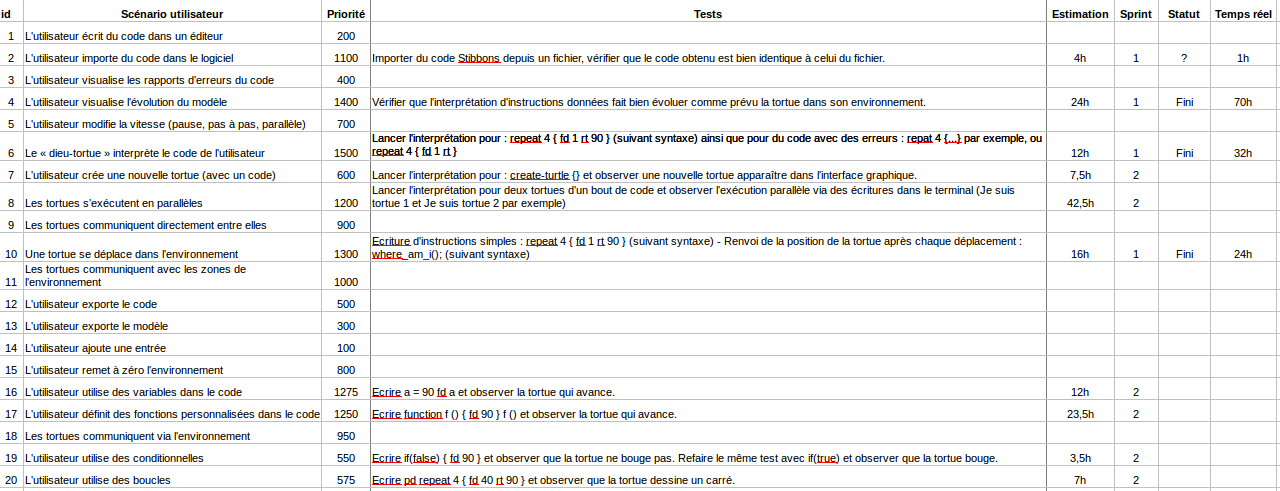
\includegraphics[scale=0.35]{doc/gestionProjet/backlogv1.png}
\end{figure}


\setcellgapes{1pt}
\makegapedcells
%\newcolumntype{R}[1]{>{\raggedleft\arraybackslash }b{#1}}
%\newcolumntype{L}[1]{>{\raggedright\arraybackslash }b{#1}}
%\newcolumntype{C}[1]{>{\centering\arraybackslash }b{#1}}
\begin{table}
\centering
\begin{tabular}{*{8}{c|}}
\hline
id & Scénario utilisateur &  Priorité &  Tests & Estimations & Sprint & Status & Temps réel  \\
\hline
1 & L'utilisateur écrit du code dans un éditeur &  200
\hline
2 & L'utilisateur importe du code dans le logiciel & 1100 & Importer du code Stibbons depuis un fichier, vérifier que le code obtenu est bien identique à celuit du fichier & 4h & 1 & ? & 1h
\hline
3 & L'utilisateur visualise les rapports d'erreurs du code & 400 &
\hline
4 & L'utilisateur visualise l'évolution du modèle & 1400 & Vérifier que l'interprétation d'instructions données fait bien évoluer comme prévu la tortue dans son environnement & 24h & 1 & Fini & 70h
\hline
5 & L'utilisateur modifie la vitesse (pause ,pas à pas, parallèle) & 700
\hline
6 & Le «dieu-tortue» interprète le code de l'utilisateur & 1500 & Lancer l'interprétation pour : repeat 4 {fd 4 rt 90} (suivant syntaxe) ainsi que pour du code avec des erreurs : repat 4{...} par exemple, ou repeat 4 {fd 1 rt} & 12h & 1 & Fini & 32h
\hline
7 & L'utilisateur
\end{tabular}
\caption{Backlog Initial}
\label{tab1}
\end{table}
